\subsection{Revision Table}
\hspace{-3cm}
\begin{table}[h!]
  \centering
  \begin{tabular}{ | m{4cm} | m{4cm} | m{5cm} | m{4cm} | }
    %% TITLE
    \hline
    \textbf{Circuit Diagram} & \textbf{Name, Objectives and Function} & \textbf{Key Equations} & \textbf{Assumptions} \\ 
    \hline
    % %% NFET CURRENT SOURCE
    \center 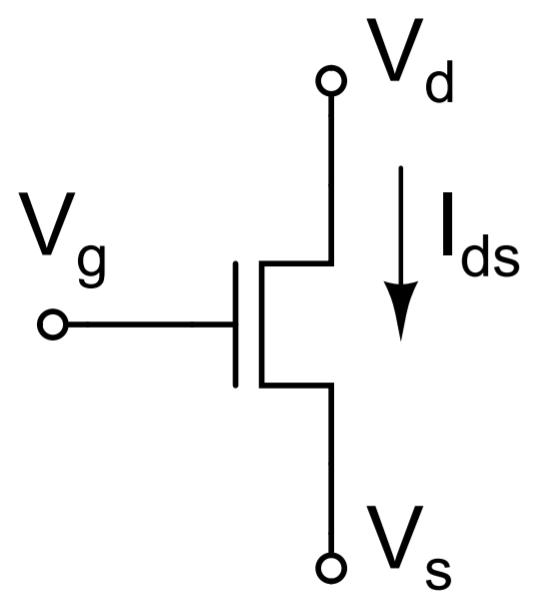
\includegraphics[width=0.7\linewidth]{Figures/N_FET_Current_Source.PNG}
    &
    \textbf{NFET Current Source}: \newline Control current in a device through applied voltage.
    &
    \centering In Saturation: \newline \newline \begin{equation*}I_{ds} =  I_{n0} e^{\frac{\kappa_{n}V_g - V_s}{U_T}}\end{equation*} \newline \newline
    \centering Not in Saturation: \newline \newline \begin{equation*}I_{ds} = I_{n0} e^{\frac{\kappa_{n}V_g}{U_T}}(e^\frac{-V_s}{U_T} - e^\frac{-V_d}{U_T})\end{equation*}
    & 
    \begin{itemize}
        \item Neglecting Early Effect (in Saturation)
        \item Neglecting Back Gate Effect
        \item Assuming $W/L = 1$
        \item Operating in Subthreshold
        \item Probably a lot more assumptions 
    \end{itemize}
    
    
    %% PFET CURRENT SOURCE
    \\ \hline
    \center 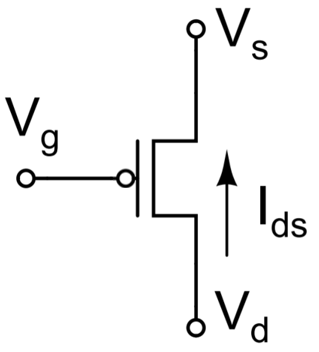
\includegraphics[width=0.7\linewidth]{Figures/pFET_Current_Source.PNG}
    &
    \textbf{PFET Current Source}: \newline  Control current in a device through applied voltage.
    &
    \centering In Saturation: \newline \newline \begin{equation*}I_{sd} = I_{p0} e^{\frac{-\kappa_p V_g + V_s}{U_T}}\end{equation*} \newline \newline
    \centering Not in Saturation: \newline \newline \begin{equation*}I_{sd} = I_{p0} e^{\frac{-\kappa_p V_g + V_s}{U_T}} (1 - e^{\frac{V_{ds}}{U_T}})\end{equation*}
    & 
    \begin{itemize}
        \item Neglecting Early Effect (in Saturation)
        \item Neglecting Back Gate Effect
        \item Assuming $W/L = 1$
        \item Operating in Subthreshold
        \item Probably a lot more assumptions 
    \end{itemize}
    
    \\ \hline
    
  \end{tabular}
\end{table}
